
\section{The FCI Hamiltonian}
Let us define two Fock spaces $F^\alpha$ and $F^\beta$ with K orbitals each and $N_\alpha$ and $N_\beta$ electrons respectively.
Let us then define Fock space $F^x$ as : $F^\alpha  \bigotimes F^\beta$ in which we let the FCI Hamiltonian operate:
\begin{equation}\label{eq:ham}
    \hat{\mathcal{H}}_\text{elec} = \sum_{pq}^K k_{pq} \hat{E}_{pq} + \frac{1}{2} \sum_{pqrs}^K g_{pqrs} \hat{E}_{pq} \hat{E}_{rs}
\end{equation}
However we can deconstruct this as 3 simplified Hamiltonians working in $F^\alpha$, $F^\beta$ and $F^x$.
\begin{align}
    \hat{\mathcal{H}}^{\alpha}_\text{elec} &= \sum_{pq}^K k_{pq} \hat{E}^{\alpha}_{pq} + \frac{1}{2} \sum_{pqrs}^K g_{pqrs} \hat{E}_{pq}^{\alpha} \hat{E}^{\alpha}_{rs} \label{eq:halpha} \\
    \hat{\mathcal{H}}^{\beta}_\text{elec} &= \sum_{pq}^K k_{pq} \hat{E}^{\beta}_{pq} + \frac{1}{2} \sum_{pqrs}^K g_{pqrs} \hat{E}_{pq}^{\beta} \hat{E}^{\beta}_{rs} \label{eq:hbeta} \\
    \hat{\mathcal{H}}^{x}_\text{elec} &= \sum_{pqrs}^K g_{pqrs} \hat{E}_{pq}^{\alpha} \hat{E}^{\beta}_{rs} \label{eq:hmix}
\end{align}
This allows us to work with relative addresses for both spin functions and then order them logically in your total Fock space. Given the nature of our Hamiltonian (total operators do not affect spin) we can write an ONV as two ONVs from the two seperate Fock spaces. $\ket{ONV} = \ket{ONV_\alpha ONV_\beta}$. Choose one of the ONVs to be major and the other minor. If for example your $\alpha$ Fock space is major your $ONV_\alpha$ will permutate after a full permutation of your $ONV_\beta$ which are $\beta$ Fock space dimension permutations.
We define $\textbf{dim}_\alpha$ as the $\alpha$ Fock space dimension and $\textbf{dim}_\beta$ as the $\beta$ Fock space dimension and the total dimension $\textbf{dim}_{total} = \textbf{dim}_\alpha * \textbf{dim}_\beta$. \\
Let us also define the following intermediates As found in Helgaker (ref) for future reference:
\begin{align}
\sigma^{\alpha pq}_{I_\alpha J_\alpha} & = \bra{I_\alpha} E^{\alpha}_{pq} \ket{J_\alpha} \label{eq:sigma} \\
\theta^{\beta pq}_{I_\beta J_\beta} & = \sum_{rs} g_{pqrs} \bra{I_\beta} E^{\beta}_{rs} \ket{J_\beta} \label{eq:theta}
\end{align}

\subsection{Constructing the Hamiltonian matrix}

Using equations (\ref{eq:halpha}) and (\ref{eq:hbeta}) we can calculate two matrixes $\textbf{H}^\alpha$ and $\textbf{H}^\beta$ of dimension $F^\alpha$ and $F^\beta$ respectively.
These can then we used in the total Hamiltonian of dimension $F^x$. As example take $F_{dim}^\alpha = 3$ and $F_{dim}^\beta = 3$:

\begin{table}[H]
  \begin{center}
\begin{tabular}{|l||l|l|l|l|l|l|l|l|l|}
\hline
 & $I_{1}^{\alpha} I_{1}^{\beta}$ & $I_{1}^{\alpha} I_{2}^{\beta}$  &  $I_{1}^{\alpha} I_{3}^{\beta}$ &  $I_{2}^{\alpha} I_{1}^{\beta}$ & $I_{2}^{\alpha} I_{2}^{\beta}$  &  $I_{2}^{\alpha} I_{3}^{\beta}$ &  $I_{3}^{\alpha} I_{1}^{\beta}$ &  $I_{3}^{\alpha} I_{2}^{\beta}$ & $I_{3}^{\alpha} I_{3}^{\beta}$ \\ \hline \hline
$I_{1}^{\alpha} I_{1}^{\beta}$ &  &  &  &  &  &  &  &  &  \\ \hline
$I_{1}^{\alpha} I_{2}^{\beta}$ &  &  &  &  &  &  &  &  &  \\ \hline
$I_{1}^{\alpha} I_{3}^{\beta}$ &  &  &  &  &  &  &  &  &  \\ \hline
$I_{2}^{\alpha} I_{1}^{\beta}$ &  &  &  &  &  &  &  &  &  \\ \hline
$I_{2}^{\alpha} I_{2}^{\beta}$ &  &  &  &  &  &  &  &  &  \\ \hline
$I_{2}^{\alpha} I_{3}^{\beta}$ &  &  &  &  &  &  &  &  &  \\ \hline
$I_{3}^{\alpha} I_{1}^{\beta}$ &  &  &  &  &  &  &  &  &  \\ \hline
$I_{3}^{\alpha} I_{2}^{\beta}$ &  &  &  &  &  &  &  &  &  \\ \hline
$I_{3}^{\alpha} I_{3}^{\beta}$ &  &  &  &  &  &  &  &  &  \\ \hline
\end{tabular}
\end{center}
\end{table}
\subsubsection{Spin seperated}
For a set of operators only affecting one spin function we can repeat the coupling as many times as there are permutations in the Fock space of the opposite spin. e.g.:
\begin{equation} \label{eq:coupling_alpha}
  \bra{I_\alpha I_\beta} \hat{a}^{\dagger}_{p \alpha} \hat{a}_{q \alpha} \hat{a}^{\dagger}_{r \alpha} \hat{a}_{s \alpha} \ket{J_\alpha I_\beta} \neq 0
\end{equation}
Values from  $\textbf{H}^\alpha$ and $\textbf{H}^\beta$ can then be repeated as such:
\begin{table}[H]
\begin{center}
\begin{tabular}{|l||l|l|l|l|l|l|l|l|l|}
\hline
 & $I_{1}^{\alpha} I_{1}^{\beta}$ & $I_{1}^{\alpha} I_{2}^{\beta}$  &  $I_{1}^{\alpha} I_{3}^{\beta}$ &  $I_{2}^{\alpha} I_{1}^{\beta}$ & $I_{2}^{\alpha} I_{2}^{\beta}$  &  $I_{2}^{\alpha} I_{3}^{\beta}$ &  $I_{3}^{\alpha} I_{1}^{\beta}$ &  $I_{3}^{\alpha} I_{2}^{\beta}$ & $I_{3}^{\alpha} I_{3}^{\beta}$ \\ \hline \hline
$I_{1}^{\alpha} I_{1}^{\beta}$ & $\text{H}^{\alpha}_{11}$ &  &  & $\text{H}^{\alpha}_{12}$ &  &  & $\text{H}^{\alpha}_{13}$ &  &  \\ \hline
$I_{1}^{\alpha} I_{2}^{\beta}$ &  & $\text{H}^{\alpha}_{11}$ &  &  & $\text{H}^{\alpha}_{12}$ &  &  & $\text{H}^{\alpha}_{13}$  &  \\ \hline
$I_{1}^{\alpha} I_{3}^{\beta}$ &  &  & $\text{H}^{\alpha}_{11}$ &  &  & $\text{H}^{\alpha}_{12}$ &  &  & $\text{H}^{\alpha}_{13}$ \\ \hline
$I_{2}^{\alpha} I_{1}^{\beta}$ & $\text{H}^{\alpha}_{21}$ &  &  & $\text{H}^{\alpha}_{22}$ &  &  & $\text{H}^{\alpha}_{23}$ &  &  \\ \hline
$I_{2}^{\alpha} I_{2}^{\beta}$ &  & $\text{H}^{\alpha}_{21}$ &  &  & $\text{H}^{\alpha}_{22}$ &  &  & $\text{H}^{\alpha}_{23}$ &  \\ \hline
$I_{2}^{\alpha} I_{3}^{\beta}$ &  &  &  $\text{H}^{\alpha}_{21}$&  &  & $\text{H}^{\alpha}_{22}$ &  &  & $\text{H}^{\alpha}_{23}$ \\ \hline
$I_{3}^{\alpha} I_{1}^{\beta}$ & $\text{H}^{\alpha}_{31}$ &  &  & $\text{H}^{\alpha}_{32}$ &  &  & $\text{H}^{\alpha}_{33}$ &  &  \\ \hline
$I_{3}^{\alpha} I_{2}^{\beta}$ &  & $\text{H}^{\alpha}_{31}$ &  &  & $\text{H}^{\alpha}_{32}$ &  &  & $\text{H}^{\alpha}_{33}$ &  \\ \hline
$I_{3}^{\alpha} I_{3}^{\beta}$ &  &  & $\text{H}^{\alpha}_{31}$ &  &  & $\text{H}^{\alpha}_{32}$ &  &  & $\text{H}^{\alpha}_{33}$ \\ \hline
\end{tabular}
\end{center}
\end{table}

and

\begin{table}[H]
\begin{center}
\begin{tabular}{|l||l|l|l|l|l|l|l|l|l|}
\hline
 & $I_{1}^{\alpha} I_{1}^{\beta}$ & $I_{1}^{\alpha} I_{2}^{\beta}$  &  $I_{1}^{\alpha} I_{3}^{\beta}$ &  $I_{2}^{\alpha} I_{1}^{\beta}$ & $I_{2}^{\alpha} I_{2}^{\beta}$  &  $I_{2}^{\alpha} I_{3}^{\beta}$ &  $I_{3}^{\alpha} I_{1}^{\beta}$ &  $I_{3}^{\alpha} I_{2}^{\beta}$ & $I_{3}^{\alpha} I_{3}^{\beta}$ \\ \hline \hline
$I_{1}^{\alpha} I_{1}^{\beta}$ & $\text{H}^{\beta}_{11}$ & $\text{H}^{\beta}_{12}$ & $\text{H}^{\beta}_{13}$ &  &  &  &  &  &  \\ \hline
$I_{1}^{\alpha} I_{2}^{\beta}$ & $\text{H}^{\beta}_{21}$ & $\text{H}^{\beta}_{22}$ & $\text{H}^{\beta}_{23}$ &  &  &  &  &  &  \\ \hline
$I_{1}^{\alpha} I_{3}^{\beta}$ & $\text{H}^{\beta}_{31}$ & $\text{H}^{\beta}_{32}$ & $\text{H}^{\beta}_{33}$ &  &  &  &  &  &  \\ \hline
$I_{2}^{\alpha} I_{1}^{\beta}$ &  &  &  &  $\text{H}^{\beta}_{11}$ & $\text{H}^{\beta}_{12}$ & $\text{H}^{\beta}_{13}$  &  &  &  \\ \hline
$I_{2}^{\alpha} I_{2}^{\beta}$ &  &  &  &  $\text{H}^{\beta}_{21}$ & $\text{H}^{\beta}_{22}$ & $\text{H}^{\beta}_{23}$  &  &  &  \\ \hline
$I_{2}^{\alpha} I_{3}^{\beta}$ &  &  &  &  $\text{H}^{\beta}_{31}$ & $\text{H}^{\beta}_{32}$ & $\text{H}^{\beta}_{33}$  &  &  &  \\ \hline
$I_{3}^{\alpha} I_{1}^{\beta}$ &  &  &  &  &  &  &  $\text{H}^{\beta}_{11}$ & $\text{H}^{\beta}_{12}$ & $\text{H}^{\beta}_{13}$ \\ \hline
$I_{3}^{\alpha} I_{2}^{\beta}$ &  &  &  &  &  &  &  $\text{H}^{\beta}_{21}$ & $\text{H}^{\beta}_{22}$ & $\text{H}^{\beta}_{23}$  \\ \hline
$I_{3}^{\alpha} I_{3}^{\beta}$ &  &  &  &  &  &  &  $\text{H}^{\beta}_{31}$ & $\text{H}^{\beta}_{32}$ & $\text{H}^{\beta}_{33}$  \\ \hline
\end{tabular}
\end{center}
\end{table}
\subsubsection{Spin mixed}
For $\textbf{H}^X$ using the intermediates (\ref{eq:sigma}) and (\ref{eq:theta})

We find for each $pq$ pair:
\begin{table}[H]
\begin{center}
\begin{tabular}{|l|l|l|l|l|l|l|l|l|l|}
\hline
 &   $I_{1}^{\alpha} I_{1}^{\beta}$ & $I_{1}^{\alpha} I_{2}^{\beta}$  &  $I_{1}^{\alpha} I_{3}^{\beta}$ &  $I_{2}^{\alpha} I_{1}^{\beta}$ & $I_{2}^{\alpha} I_{2}^{\beta}$  &  $I_{2}^{\alpha} I_{3}^{\beta}$ &  $I_{3}^{\alpha} I_{1}^{\beta}$ &  $I_{3}^{\alpha} I_{2}^{\beta}$ & $I_{3}^{\alpha} I_{3}^{\beta}$ \\ \hline \hline
 $I_{1}^{\alpha} I_{1}^{\beta}$ & \multicolumn{3}{l|}{\multirow{3}{*}{}} & \multicolumn{3}{l|}{\multirow{3}{*}{}} & \multicolumn{3}{l|}{\multirow{3}{*}{}} \\ \cline{1-1}
 $I_{1}^{\alpha} I_{2}^{\beta}$ & \multicolumn{3}{c|}{$\sigma^{\alpha pq}_{11} * \theta^{\beta pq}$}                  & \multicolumn{3}{c|}{$\sigma^{\alpha pq}_{12} * \theta^{\beta pq}$}                  & \multicolumn{3}{c|}{$\sigma^{\alpha pq}_{13} * \theta^{\beta pq}$}                \\ \cline{1-1}
 $I_{1}^{\alpha} I_{3}^{\beta}$ & \multicolumn{3}{l|}{}                  & \multicolumn{3}{l|}{}                  & \multicolumn{3}{l|}{}                  \\ \hline
 $I_{2}^{\alpha} I_{1}^{\beta}$ & \multicolumn{3}{l|}{\multirow{3}{*}{}} & \multicolumn{3}{l|}{\multirow{3}{*}{}} & \multicolumn{3}{l|}{\multirow{3}{*}{}} \\ \cline{1-1}
 $I_{2}^{\alpha} I_{2}^{\beta}$& \multicolumn{3}{c|}{$\sigma^{\alpha pq}_{21} * \theta^{\beta pq}$}                & \multicolumn{3}{c|}{$\sigma^{\alpha pq}_{22} * \theta^{\beta pq}$}                 & \multicolumn{3}{c|}{$\sigma^{\alpha pq}_{23} * \theta^{\beta pq}$}           \\ \cline{1-1}
 $I_{2}^{\alpha} I_{3}^{\beta}$ & \multicolumn{3}{l|}{}                  & \multicolumn{3}{l|}{}                  & \multicolumn{3}{l|}{}                  \\ \hline
 $I_{3}^{\alpha} I_{1}^{\beta}$ & \multicolumn{3}{l|}{\multirow{3}{*}{}} & \multicolumn{3}{l|}{\multirow{3}{*}{}} & \multicolumn{3}{l|}{\multirow{3}{*}{}} \\ \cline{1-1}
 $I_{3}^{\alpha} I_{2}^{\beta}$& \multicolumn{3}{c|}{$\sigma^{\alpha pq}_{31} * \theta^{\beta pq}$}                  & \multicolumn{3}{c|}{$\sigma^{\alpha pq}_{32} * \theta^{\beta pq}$}                 & \multicolumn{3}{c|}{$\sigma^{\alpha pq}_{33} * \theta^{\beta pq}$}               \\ \cline{1-1}
 $I_{3}^{\alpha} I_{3}^{\beta}$ & \multicolumn{3}{l|}{}                  & \multicolumn{3}{l|}{}                  & \multicolumn{3}{l|}{}                  \\ \hline
\end{tabular}
\end{center}
\end{table}

\subsection{Hamiltonian matrix vector product}
We can perform similar operations for the matrix vector product.
A vectors in the total Fock space can be stored as:
\begin{center}
\begin{tabular}{|l|l||l|}
\hline
$I_{\alpha}$ & $I_{\beta}$ & $I_{\textbf{total}}$ \\ \hline
$I_1$ & $I_1$ & $I_1$ \\ \hline
$I_1$ & $I_2$ & $I_2$ \\ \hline
$I_1$ & $I_3$ & $I_3$ \\ \hline
$I_1$ & $I_{...}$ & $I_{...}$ \\ \hline
$I_1$ & $I_{\textbf{dim}_\beta}$ & $I_{\textbf{dim}_\beta}$ \\ \hline
$I_2$ & $I_{1}$ & $I_{\textbf{dim}_\beta + 1}$ \\ \hline
$I_2$ & $I_{2}$ & $I_{\textbf{dim}_\beta + 2}$ \\ \hline
$I_{...}$ & $I_{...}$ & $I_{... * \textbf{dim}_\beta + ...}$ \\ \hline
$I_{\textbf{dim}_\alpha}$ & $I_{\textbf{dim}_\beta}$ & $I_{\textbf{dim}_{total}}$ \\ \hline
\end{tabular}
\end{center}
Rudimentary approach to performing the matrix vector product for a none storable Hamiltonian can be done as follows (where P is the vector resulting from the product and X is the vector partaking in the product):
\begin{align}
  \text{P}_{I} = \sum_J \text{H}_{IJ} * \text{X}_{J} \\
  \text{P}_{J} = \sum_I \text{H}_{JI} * \text{X}_{I}
\end{align}
Where $\text{Hamiltonian}_{JI} = \text{Hamiltonian}_{IJ}$ (or $\text{Hamiltonian}_{JI} = \text{Hamiltonian}_{IJ}^*$ when working complex). Allowing for the upperdiagonal approach (for I coupling to J one finds J coupling to I)

\subsubsection{Evaluations Seperated by Spin}
We can calculate a portion of P (all one-electron and part of the two-electron (only the same spin) evaluations), $\text{P}^{\alpha}$ and $\text{P}^{\beta}$.
Where we now define $\text{P} = \text{P}^{\alpha \beta} + \text{P}^{\alpha} + \text{P}^{\beta}$ with $\text{P}^{\alpha \beta}$ exclusively operator combinations working on both spin functions simultaneously.
Equation (\ref{eq:coupling_alpha}) holds for any $I_\beta$.
Allowing to re-use calculated Hamiltonian elements related to the coupling.
\begin{align}
  \forall I_\beta: \text{P}^{\alpha}_{I_\alpha * \textbf{dim}_\beta + I_\beta} = \sum_{J_\alpha > I_\alpha} \text{H}^{\alpha}_{I_\alpha J_\alpha} * \text{X}_{J_\alpha * \textbf{dim}_\beta + I_\beta} \\
  \forall I_\beta: \text{P}^{\alpha}_{J_\alpha * \textbf{dim}_\beta + I_\beta} = \sum_{I_\alpha > J_\alpha} \text{H}^{\alpha}_{J_\alpha I_\alpha} * \text{X}_{I_\alpha * \textbf{dim}_\beta + I_\beta}
\end{align}
Base-line implementation (with a for loop) will result significant difference in execution speed for both spin functions.
As an example we have an FCI calculation with $K=12$ molecular orbitals and 6 $\alpha$ electrons and 6 $\beta$ electrons.
Yielding an Alpha and Beta Fock space of dimenion 924 and a total dimension of 853.776k where alpha is major as in the vector example above.
Calculating all couplings with Alpha and perfoming the matvec takes: $249 ms$ versus Beta: $2561 ms$.
The alpha matvec is a lot cheaper because it gets repeated in an uninterrupted sequencel matter, versus beta which repeats with a large interval (the dimenion of the alpha Fock space) causing cache misses. This was solved using the Eigen3 (ref EIGEN) API for efficiently performing the matvec in a vectorized matter. (There is no motivation other than educational to attempt to write a library with similar functionallity and performance as Eigen3 by yourself)

The resulting vector and the vector from the product can both be mapped to a matrix representation.

\begin{equation}
\begin{bmatrix} \label{eq:matrixrep}
    I^{\alpha}_1 I^{\beta}_1 & I^{\alpha}_1 I^{\beta}_2  & I^{\alpha}_1 I^{\beta}_{...} & \dots  & I^{\alpha}_1 I^{\beta}_{\textbf{dim}_\beta} \\
    I^{\alpha}_2 I^{\beta}_1 & I^{\alpha}_2 I^{\beta}_2  & I^{\alpha}_2 I^{\beta}_{...} & \dots  & I^{\alpha}_2 I^{\beta}_{\textbf{dim}_\beta} \\
    I^{\alpha}_{...} I^{\beta}_1 & I^{\alpha}_{...} I^{\beta}_2  & I^{\alpha}_{...} I^{\beta}_{...} & \dots  & I^{\alpha}_{...} I^{\beta}_{\textbf{dim}_\beta} \\
    \vdots & \vdots & \vdots & \ddots & \vdots \\
    I^{\alpha}_{\textbf{dim}_\alpha} I^{\beta}_1 & I^{\alpha}_{\textbf{dim}_\alpha} I^{\beta}_2  & I^{\alpha}_{\textbf{dim}_\alpha} I^{\beta}_{...} & \dots  &
    I^{\alpha}_{\textbf{dim}_\alpha} I^{\beta}_{\textbf{dim}_\beta}
\end{bmatrix}
\end{equation}
Using $\textbf{H}^{\alpha}$ and $\textbf{H}^{\beta}$ will be sparse and will only cost a fraction to store compared P and X.
Let us call $\mathcal{P}$: P mapped as the matrix in eqation (\ref{eq:matrixrep})

\begin{align}
    \forall I_\beta: \mathcal{P}^{\alpha}_{I_\alpha I_\beta} & = \sum_{J_\alpha} \text{H}^{\alpha}_{I_\alpha J_\alpha} * \mathbb{X}_{J_\alpha I_\beta} \\
    \forall I_\alpha: \mathcal{P}^{\beta}_{I_\alpha  I_\beta} & = \sum_{J_\beta} \text{H}^{\beta}_{I_\beta J_\beta} * \mathbb{X}_{I_\alpha J_\beta} \\
   \mathcal{P}^\alpha & = \text{H}^{\alpha} * \mathbb{X} \\
  \mathcal{P}^\beta & = \mathbb{X} * \text{H}^{\beta}
\end{align}
Eigen3 offers a sparse matrix module (initialize it with vector of \code{Eigen::Triplets}). One can either only fill the upperdiagonal and use
\\
 \code{Eigen::SparseMatrix::selfadjointView<upper>()}
when performing a matrix multiplication, however I have found that filling both upper and lower diagonal of the self adjoint \code{SparseMatrx} significantly reduces the execution time of the matrix multiplication.

\subsubsection{Evaluations of the two-electron mixed spin operators}

\begin{align}
\mathcal{P}^{\alpha \beta} & = \sum_{pq}  \mathcal{P}^{\alpha \beta pq} = \sum_{pq} \sigma^{\alpha pq} * \mathbb{X} * \theta^{\beta pq} \\
\sigma^{\alpha pq}_{I_\alpha J_\alpha} & =\bra{I_\alpha} E^{\alpha}_{pq} \ket{J_\alpha} \\
\theta^{\beta pq}_{I_\beta J_\beta} &  = \sum_{rs} g_{pqrs} \bra{I_\beta} E^{\beta}_{rs} \ket{J_\beta}
\end{align}

Because $g_{pqrs} = g_{qprs}$ one can include both $p,q$ and $q,p$ in a single alpha coupling matrix, allowing $\sum_p \sum_{q \geq p}$. Additionally if you want to omit diagonal calculations, simply omit any calculations where $r=s$ from the $\theta^{\beta pq}$ if $p=q$.

\subsection{Memory requirements}

Between each matrix vector product we have some required storage (P and X, in our code also the diagonal) and some optional.
Minimal storage (in arbitrary units) required is approximately: $3 * \text{dim}_{total} = 3 * \binom{K}{N_\alpha}\binom{K}{N_\beta}$
For the optional intermediates we need:
\begin{align}
  \text{H}^{\alpha} &= \binom{K}{N_\alpha} * \big(\frac{\binom{K-N_\alpha}{2}}{2} * (N_{\alpha}^2-N_\alpha) + (K-N_\alpha)*N_\alpha \big) \\
  \text{H}^{\beta} &= \binom{K}{N_\beta} * \big(\frac{\binom{K-N_\beta}{2}}{2} * (N_{\beta}^2-N_\beta) + (K-N_\beta)*N_\beta \big) \\
  \sigma^{\alpha pq} * (K^2 - K) & \approx \binom{K-1}{N_\alpha-1} * (K^2 - K) \\
  \theta^{\beta pq} * (K^2) & \approx \binom{K}{N_\beta} * (K-N_\beta)*N_\beta * K^2
\end{align}

% \begin{center}
%
% \begin{figure}
%   \centering
%   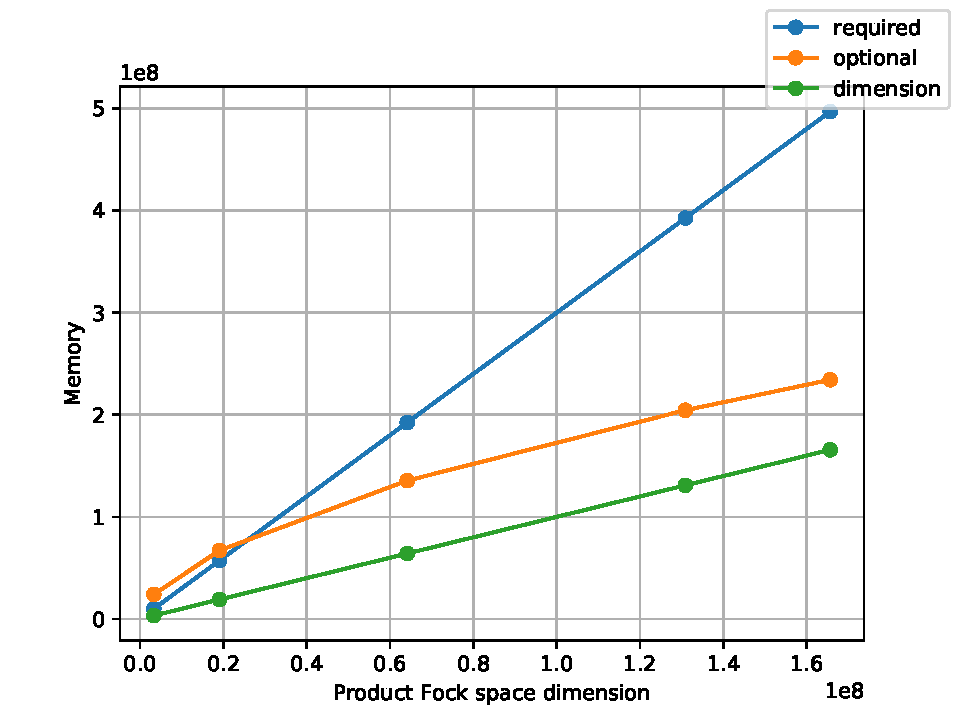
\includegraphics[width=10cm]{graphs/K=16.pdf}
%   \caption{K=16 and $N_\alpha = N_\beta [4,8[$}
%   \label{}
% \end{figure}
%
% \begin{figure}
%   \centering
%   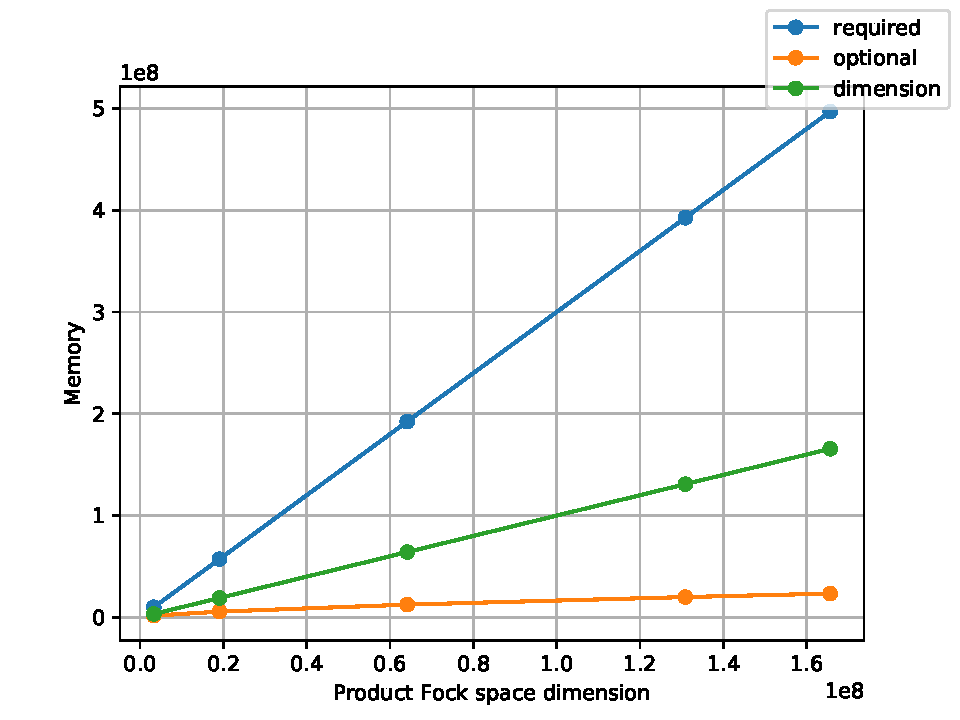
\includegraphics[width=10cm]{graphs/K=16_low.pdf}
%   \caption{K=16 and $N_\alpha = N_\beta [4,8[$ no $\theta$}
%   \label{}
% \end{figure}
%
% \begin{figure}
%   \centering
%   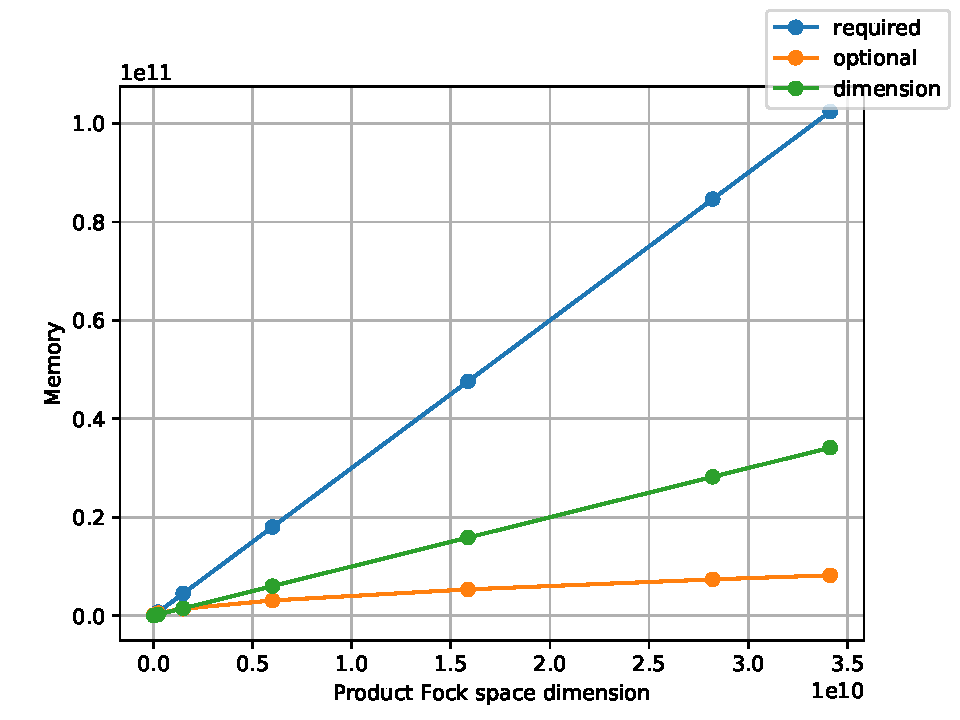
\includegraphics[width=10cm]{graphs/K=20.pdf}
%   \caption{K=20 and $N_\alpha = N_\beta [4,10[$}
%   \label{}
% \end{figure}
%
% \begin{figure}
%   \centering
%   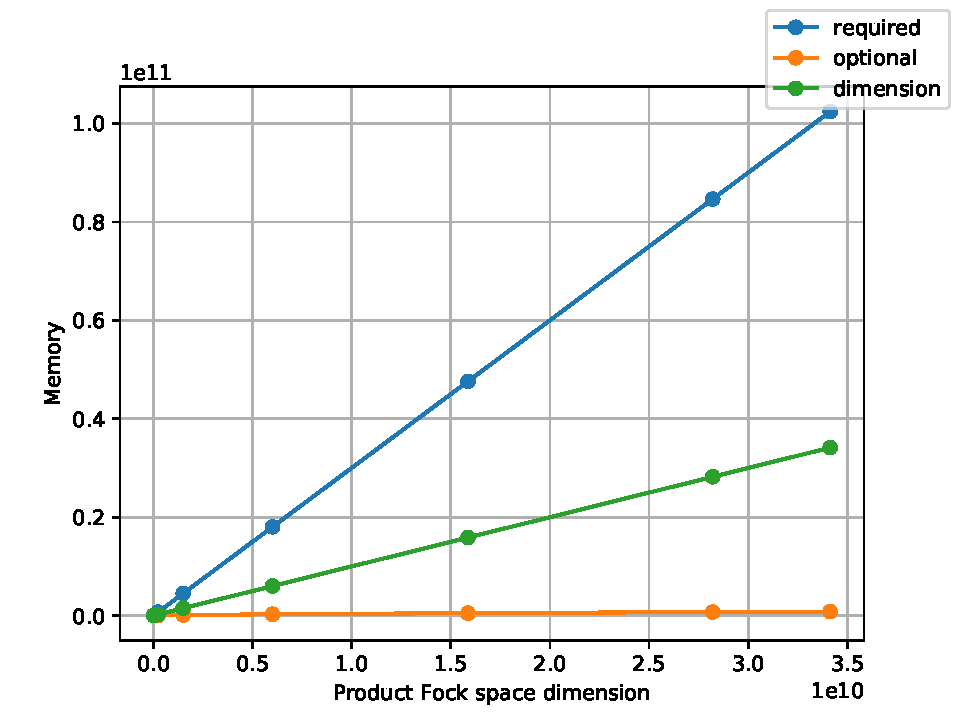
\includegraphics[width=10cm]{graphs/K=20_low.pdf}
%   \caption{K=20 and $N_\alpha = N_\beta [4,10[$  no $\theta$}
%   \label{}
% \end{figure}
%
% \begin{figure}
%   \centering
%   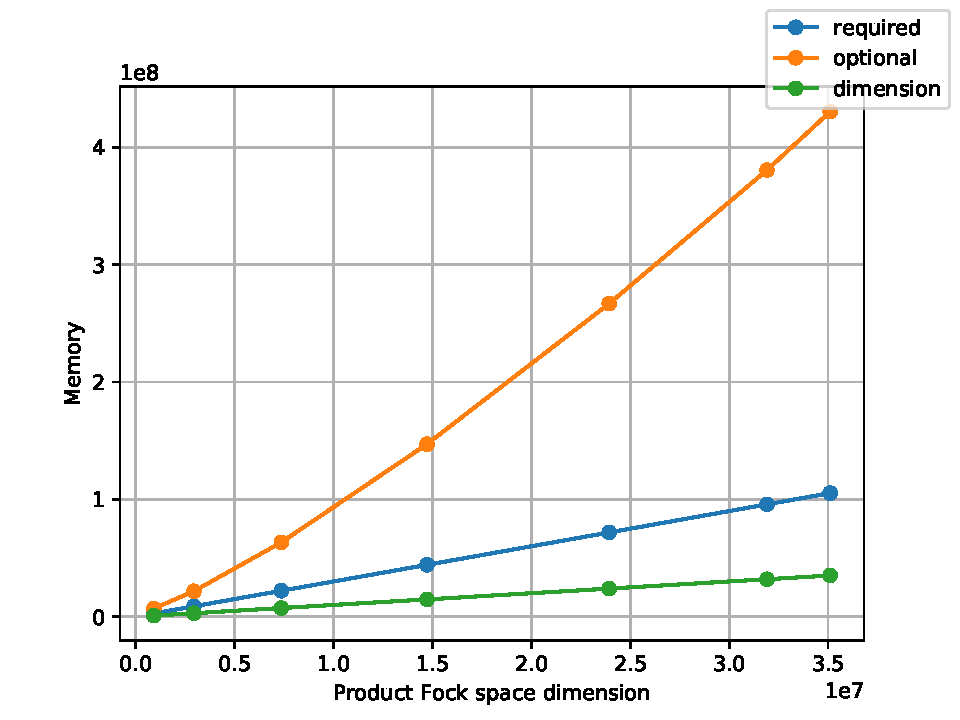
\includegraphics[width=10cm]{graphs/K=20_neq.pdf}
%   \caption{K=20 and $N_\beta = 2, N_\alpha [4,10[$}
%   \label{}
% \end{figure}
%
% \begin{figure}
%   \centering
%   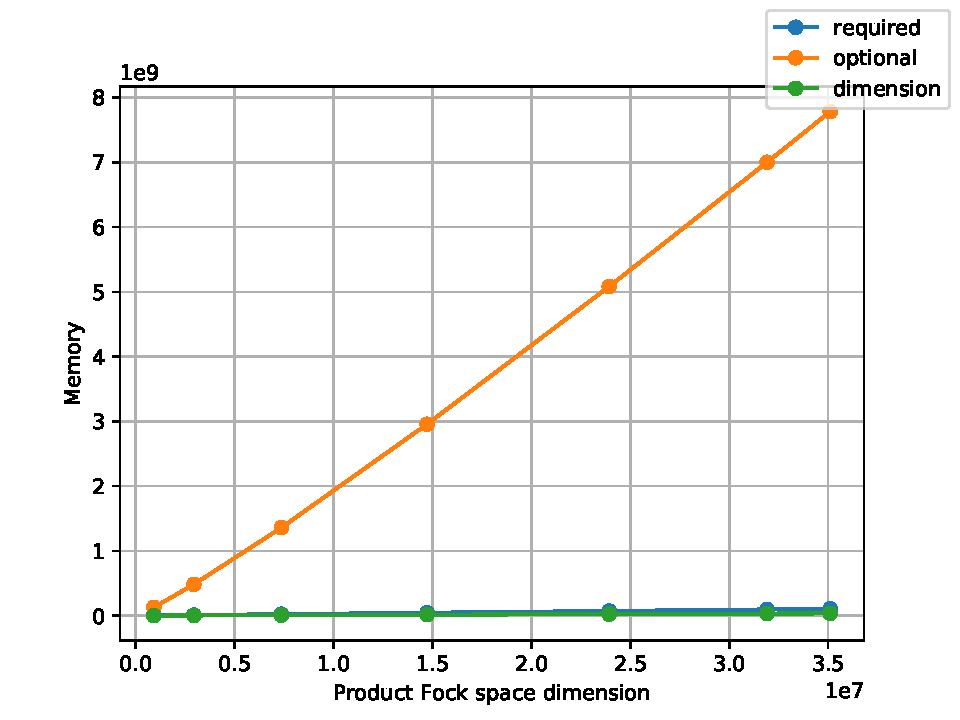
\includegraphics[width=10cm]{graphs/K=20_neq_dumb.pdf}
%   \caption{K=20 and $N_\alpha = 2, N_\beta [4,10[$}
%   \label{}
% \end{figure}
%
% \begin{figure}
%   \centering
%   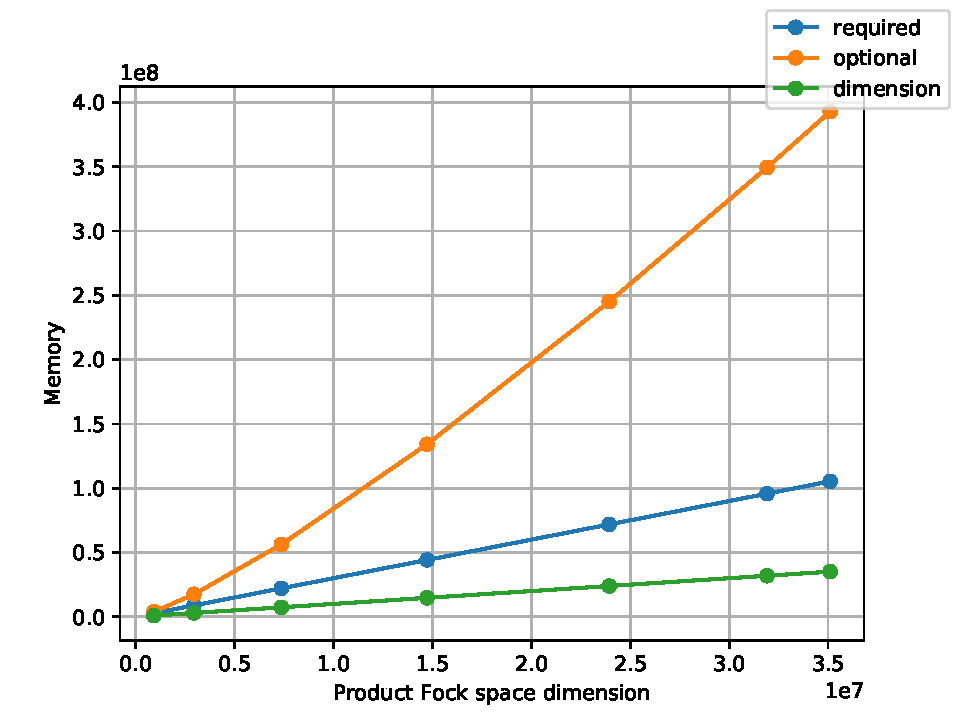
\includegraphics[width=10cm]{graphs/K=20_neq_dumb_low.pdf}
%   \caption{K=20 and $N_\alpha = 2, N_\beta [4,10[$ no $\theta$}
%   \label{}
% \end{figure}
%
% \end{center}

\subsection{Minimal two electron operator iterations}

We will focus only on the two electron operators $ \sum_{pqrs}^K g_{pqrs} \hat{a}^{\dagger}_{p} \hat{a}_{q}  \hat{a}^{\dagger}_{r} \hat{a}_{s}$. And only focus on the $\alpha$ electrons. We will therefore ignore the $\alpha$ subscript.
We require to consider operator indices for which a given ONV I does not vanish:
\begin{equation} \label{eq:address}
  \bra{I} \hat{a}^{\dagger}_{p} \hat{a}_{q} \hat{a}^{\dagger}_{r} \hat{a}_{s} = \bra{J}
\end{equation}
In which $J$ is an address larger than $I$. Reason for this is, in the event that $\ket{I}$ can be transformed in $\ket{J}$. $\ket{J}$ can also be transformed back to $\ket{I}$ yielding the same two-electron term (hermitian two-electron operators).

\begin{equation}
  (\bra{I} E_{pq} E_{rs} \ket{J})^\dagger = \bra{J} E_{sr} E_{qp} \ket{I}
\end{equation}

It is important to note, that I will base further explanations from the perspective of equation (\ref{eq:address}) where $\hat{a}^{\dagger}_{p}$ annihilates on $\bra{I}$.
\\
For the address to be larger at all times, the highest index of a creation should always be higher than the highest index of an annihilation. This is easily verified by the fact that we represent our ONVs in binary and that the addressing is based on the ordering of its integer value. Given the relation of numeric value for each index of an integer represented in binary is quadratic, the integer value of a set index is always larger than any combination of previously set indices:
\begin{equation}
  2^N - 1 = \sum^{N-1}_{i=0} 2^i
\end{equation}
Additionally we can state that the first annihiltion can always have a smaller index than the second annihiltion without skipping over any address, the same is true for the creation operators.

Regardless in which way they are executed (if they are all different indices), the address will be the same. However the order of execution can alter the expression (sign wise) and will be accompanied by a different two-electron term. Given an ONV $\bra{I}$ for which $\bra{I} \hat{a}^\dagger_p \hat{a}_q \hat{a}^\dagger_r \hat{a}_s \neq 0 $ we find that:
\begin{align}
  \bra{I} \hat{a}^\dagger_p \hat{a}_q \hat{a}^\dagger_r \hat{a}_s & = \bra{I} (\hat{a}^\dagger_p \hat{a}_s \delta_{rq} - \hat{a}^\dagger_p \hat{a}^\dagger_r \hat{a}_q \hat{a}_s) \nonumber \\
  & = \bra{I} (\hat{a}^\dagger_p  \hat{a}_s \delta_{rq} + \hat{a}^\dagger_r \hat{a}^\dagger_p \hat{a}_q \hat{a}_s) \nonumber \\
  & = \bra{I} (\hat{a}^\dagger_p  \hat{a}_s \delta_{rq} + \hat{a}^\dagger_r \hat{a}_s \delta_{pq} - \hat{a}^\dagger_r \hat{a}_q \hat{a}^\dagger_p \hat{a}_s) \label{eq:equals} \\
  & \text{IF p,q,r,s $\neq$} \nonumber \\
  & = - \bra{I}(\hat{a}^\dagger_r \hat{a}_q \hat{a}^\dagger_p \hat{a}_s )\\
  & = \bra{I} (\hat{a}^\dagger_r \hat{a}_s \hat{a}^\dagger_p \hat{a}_q ) \\
  & = - \bra{I} (\hat{a}^\dagger_p \hat{a}_s \hat{a}^\dagger_r \hat{a}_q)
\end{align}
So for the \textit{p,q,r,s $\neq$} case, we can enforce : $p<r$, $q<s$ for symmetries and anti-symmetries, and $s > r$ upper diagonal to not generate redundant addresses. This leaves us with limited combinations:

\begin{enumerate}
  \item $p > q$ ($s > r > p$)
  \item $p < q$
  \begin{itemize}
    \item $r > q$ ($s > r$)
    \item $q > r$ ($s > q$)
  \end{itemize}
\end{enumerate}
For inplace annihila-crea- and crea-annihila-tions, the rules are slightly different, because creation annihilation operators with the same index cancel each other out. Therefore the non-annihiltion bound creation index has to be larger than the non-creation bound annihiltion index to produce larger addresses (the rules for one-electron evaluation).

\begin{enumerate}
  \item $p = q$, $s > r$
  \item $q = r$, $s > p$
\end{enumerate}
These have some implication for symmetry and anti-symmetry equations such as equation (\ref{eq:equals}) as $\delta$ is not always zero:


\begin{align}
   \bra{I}  \hat{a}^\dagger_p \hat{a}_q \hat{a}^\dagger_r \hat{a}_s & =   \bra{I} (\hat{a}^\dagger_p \hat{a}_s \delta_{rq} + \hat{a}^\dagger_r  \hat{a}_s \delta_{pq} - \hat{a}^\dagger_r \hat{a}_q \hat{a}^\dagger_p \hat{a}_s) \\
  & =   \bra{I} (\hat{a}^\dagger_p \hat{a}_s \delta_{rq} + \hat{a}^\dagger_r \hat{a}_s \delta_{pq} - \hat{a}^\dagger_r \hat{a}_q  \delta_{sp} - \hat{a}^\dagger_r \hat{a}_s \delta_{pq} + \hat{a}^\dagger_r \hat{a}_s \hat{a}^\dagger_p \hat{a}_q) \\
  & =   \bra{I} (\hat{a}^\dagger_p \hat{a}_q \delta_{rs} + \hat{a}^\dagger_p \hat{a}_s \delta_{qr} - \hat{a}^\dagger_p \hat{a}_s \hat{a}^\dagger_r \hat{a}_q)
\end{align}

\textbf{p = q:}
For $p = q$ we can also see that for $s = q \iff r = q$ ortherwise we would have a double creation on the same index without an annihilation on that same index, which is a vanishing operation sequence. However this does not alter the address (diagonal contribution) and is ignored in the algorithm. Hence we state that $ s \neq p, q, r $ This simplifies the equations:

\begin{align}
  \bra{I}  \hat{a}^\dagger_p \hat{a}_p \hat{a}^\dagger_r \hat{a}_s & =  \bra{I} (\hat{a}^\dagger_p \hat{a}_s \delta_{rp} + \hat{a}^\dagger_r  \hat{a}_s - \hat{a}^\dagger_r \hat{a}_p \hat{a}^\dagger_p \hat{a}_s) \\
  & =   \bra{I} (\hat{a}^\dagger_p \hat{a}_s \delta_{rp} + \hat{a}^\dagger_r \hat{a}_s \hat{a}^\dagger_p \hat{a}_p) \\
  & =   \bra{I} (\hat{a}^\dagger_p \hat{a}_s \delta_{pr} - \hat{a}^\dagger_p \hat{a}_s \hat{a}^\dagger_r \hat{a}_p)
\end{align}
We can then discriminate between $r = p$ :

\begin{align}
    \bra{I} \hat{a}^\dagger_p \hat{a}_p \hat{a}^\dagger_p \hat{a}_s & =   \bra{I} (\hat{a}^\dagger_p \hat{a}_s + \hat{a}^\dagger_p \hat{a}_s - \hat{a}^\dagger_p \hat{a}_p \hat{a}^\dagger_p \hat{a}_s ) \\
  & =   \bra{I} (\hat{a}^\dagger_p \hat{a}_s + \hat{a}^\dagger_p \hat{a}_s \hat{a}^\dagger_p \hat{a}_p) \label{eq:vanish1} \\
  & =   \bra{I} (\hat{a}^\dagger_p \hat{a}_s - \hat{a}^\dagger_p \hat{a}_s \hat{a}^\dagger_p \hat{a}_p) \label{eq:vanish2}
\end{align}
We see in equation (\ref{eq:vanish1}) and (\ref{eq:vanish2}) that last term annihilates $p$, then operator on index $s$ does strictly not create on index $p$ and index $p$ is annihilated again, thus this term vanishes:

\begin{equation}
 \bra{I}  \hat{a}^\dagger_p \hat{a}_p \hat{a}^\dagger_p \hat{a}_s = \bra{I} \hat{a}^\dagger_p \hat{a}_s
\end{equation}
For $r \neq p$:
\begin{align}
    \bra{I} \hat{a}^\dagger_p \hat{a}_p \hat{a}^\dagger_r \hat{a}_s & =   \bra{I} ( \hat{a}^\dagger_r  \hat{a}_s - \hat{a}^\dagger_r \hat{a}_p \hat{a}^\dagger_p \hat{a}_s ) \nonumber \\
  & =   \bra{I} (\hat{a}^\dagger_r  \hat{a}_s) \label{eq:rneqp}\\
  & =   \bra{I} ( \hat{a}^\dagger_r \hat{a}_s \hat{a}^\dagger_p \hat{a}_p) \\
  & = -   \bra{I} (\hat{a}^\dagger_p \hat{a}_s \hat{a}^\dagger_r \hat{a}_p)
\end{align}
Where se see that for equation (\ref{eq:rneqp}) the second term vanished, as the initial term is assumend non-vanishing.

\textbf{q=r:}
We only cover $p \neq r$ as we assume tha $r$ starts unoccupied as opposed to the previous section (\ref{p=q}).
\begin{align}
  \bra{I} \hat{a}^\dagger_p \hat{a}_r \hat{a}^\dagger_r \hat{a}_s & =   \bra{I} (\hat{a}^\dagger_p \hat{a}_s - \hat{a}^\dagger_r \hat{a}_r \hat{a}^\dagger_p \hat{a}_s) \nonumber \\
  & =   \bra{I} \hat{a}^\dagger_p \hat{a}_s  \\
  & =   \bra{I} (\hat{a}^\dagger_p \hat{a}_s + \hat{a}^\dagger_r \hat{a}_s \delta_{pr} - \hat{a}^\dagger_r \hat{a}_r  \delta_{sp} - \hat{a}^\dagger_r \hat{a}_s \delta_{pr} + \hat{a}^\dagger_r \hat{a}_s \hat{a}^\dagger_p \hat{a}_r) \\
  & =   \bra{I} (\hat{a}^\dagger_p \hat{a}_r \delta_{rs} + \hat{a}^\dagger_p \hat{a}_s - \hat{a}^\dagger_p \hat{a}_s \hat{a}^\dagger_r \hat{a}_r)
\end{align}
Which simplifies to:
\begin{equation}
    \bra{I} \hat{a}^\dagger_p \hat{a}_r \hat{a}^\dagger_r \hat{a}_s =   \bra{I} \hat{a}^\dagger_p \hat{a}_s
\end{equation}


\subsubsection{Summary for the Hamiltonian}
In short this we shall sum up what appears to be the minimal amount of operators required to retrieve all information for the Hamiltonian for the two-electron (same spin) operators.
The value:
\begin{equation}
  \frac{1}{2} (g_{pqrs} + g_{rspq} - g_{rqps} - g_{psrq})
\end{equation}
 Can be retrieved for any of the follwing non-vanishing operator sequence combinations yielding a higher and the same (thus non redundant) address for a given $\bra{I}$:
\begin{enumerate}
  \item $s > r > p > q$
  \item $s > r > q > p$
  \item $s > q > r > p$
\end{enumerate}
For every occupied index $x$ in an ONV:
\begin{equation}
  \frac{1}{2} (g_{xxpq} + g_{pqxx} - g_{xpqx})
\end{equation}
We can also see that for $p=x$ we arrive at:
\begin{equation}
  \frac{1}{2} (g_{xxxq})
\end{equation}
For every unnocupied index $y$ ($p \neq y$) in an ONV:
\begin{equation}
  \frac{1}{2} (g_{pyyq})
\end{equation}
Where for both cases $p<q$.
